\documentclass{article}

\usepackage{tikz}
\usetikzlibrary{arrows,calc,decorations.markings}

\begin{document}
\pgfarrowsdeclarecombine{|<}{>|}{latex}{latex}{|}{|}
\def\Dimline[#1][#2][#3]{
    %\node at (0,0) {"test: #1 - #2 ..."};
    \begin{scope}[>=latex] % redef arrow for dimension lines
        \draw[|<->|,
        decoration={markings, % switch on markings
                mark=at position 0.5 with {\node[gray] at (0,0.25) {\tiny{#3}};},
        },
        postaction=decorate] #1 -- #2 ;
    \end{scope}
}

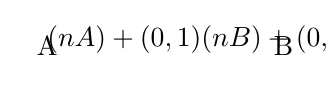
\begin{tikzpicture}

    \node at (0,0) (nA) {A};
    \node at (3,0) (nB) {B};
    \Dimline[($(nA)+(0,1)$)][($(nB)+(0,1)$)]['test'] ;

\end{tikzpicture}

\end{document}